%\documentclass[a4paper,english,12pt,twocolumn]{article}
\documentclass[a4paper,english,12pt]{article}
\usepackage[utf8]{inputenc} % Encodage du fichier
\usepackage[T1]{fontenc} % Encodage des fonts nécessaire pour le Latin
\usepackage[french]{babel} % Pour changer la langue des mots générés et choisir la bonne mise en page
\usepackage{amssymb}
\usepackage{pdflscape}
\usepackage{microtype} 
\usepackage{lmodern} % Le latin modèrne
\usepackage[top=2cm, bottom=2cm, left=2.5cm, right=1.5cm]{geometry} % Définir les marges de la page 
\usepackage[hidelinks,urlcolor=blue,unicode=true,
pdftitle={Prediction of episode's number from its summary},
pdfauthor={BELOUADAH Eden and BOUHAHA Mariem},
pdfdisplaydoctitle=true]{hyperref} % Pour les liens 
\usepackage{fancyhdr} % Pour le style de la page
\usepackage[font=it]{caption} % Rendre les titres des tableaux italiques
\usepackage{graphicx} % Pour les images
\usepackage{subcaption} % Pour mettre plusieurs images sur la même ligne
\usepackage{float} % Pour empêcher le déplacement des tableaux et des figures.
\usepackage{babelbib} % Pour changer la langue dans la bibliographie
\usepackage{amsmath} % Pour des fonctions mathématiques
\usepackage{amssymb} % Pour les symboles mathématiques
%\usepackage[onelanguage,english,longend,boxruled,algoruled,linesnumbered,algochapter,nofillcomment]{algorithm2e} %pour les algorithmes
\usepackage{multirow}
\usepackage{booktabs}
\usepackage{enumitem}
\usepackage{setspace}

\graphicspath{ {photos/} } % Spécifier le répertoire contenant les images

\DisableLigatures[f]{encoding=*}

%Active ça si tu ne veux pas les points-virgules dans les algorithmes
% \DontPrintSemicolon
 
%\renewcommand \thechapter{\Roman{chapter}} % Utiliser les numéros romans pour les chapitres

\captionsetup{labelfont=it,textfont=it,labelsep=period} % Changer le style des légendes
\AtBeginDocument{ % Changer les légendes
	\renewcommand\tablename{\itshape Tableau}
	\renewcommand{\figurename}{\itshape Figure}
	% Renommer la table des matières
	\renewcommand{\contentsname}{Sommaire}
}

% Style de l'entête et le pied de la page
\setlength{\headheight}{16pt}
\pagestyle{fancy}
\fancyhead[L]{} % Enlever la section
\fancyhead[R]{\footnotesize\slshape{\nouppercase{\leftmark}}} % Titre du chapitre en minuscule avec taille 10
\fancyfoot[C]{}
\fancyfoot[R]{\thepage} % Déplacer le numéro de la page vers la droite de la page

\fancypagestyle{plain}{
\renewcommand{\headrulewidth}{0pt}
\fancyhf{}
\fancyfoot[R]{\thepage}
}
  
% Espace entre les lignes
\linespread{1.3}

% Code pris de https://tex.stackexchange.com/a/95616/109916 et corrigé
% Début
\makeatletter
\newcommand{\emptypage}[1]{
  \cleardoublepage
  \begingroup
  \let\ps@plain\ps@empty
  \pagestyle{empty}
  #1
  \cleardoublepage
  \endgroup}
\makeatletter
% Fin


% pour changer les deux points des légendes d'algorithmes
% \SetAlgoCaptionSeparator{\unskip.}

\begin{document}
%\include{Page_de_garde}
%\include{Remerciements}
\emptypage{
%\tableofcontents
%\listoffigures
%\listoftables
}
    
\setlength{\parskip}{0.6em plus 0.1em minus 0.1em}
%\SetKwInput{KwOut}{Outpits}

% Redéfinition des chapitres et sections pour les inclure dans le sommaire
\makeatletter
%	\let\oldchapter\chapter
%	\newcommand{\@chapterstar}[1]{\cleardoublepage\phantomsection\addcontentsline{toc}{chapter}{#1}{\oldchapter*{#1}}\markboth{#1}{}}
%	\newcommand{\@chapternostar}[1]{{\oldchapter{#1}}}
%	\renewcommand{\chapter}{\@ifstar{\@chapterstar}{\@chapternostar}}
\let\oldsection\section
\newcommand{\@sectionstar}[1]{\phantomsection\addcontentsline{toc}{section}{#1}{\oldsection*{#1}}}
\newcommand{\@sectionnostar}[1]{{\oldsection{#1}}}
\renewcommand\section{\@ifstar{\@sectionstar}{\@sectionnostar}}	
\newcommand*{\rom}[1]{\expandafter\@slowromancap\romannumeral #1@}
\makeatother

\setcounter{page}{1}
%%%%%%%%%%%%%%%%%%%%%%%%%%%%%%%%%%%%%%%%%%%%%%%%%%%%%%%%%%%%%

\title{Otto Product Classification}
\author{Mariem BOUHAHA \and Eden BELOUADAH}
% \date{}
\maketitle



\section{Introduction}
Classification is an important field since it's the base of so many real world problems. This project is based on the (Otto product classification) Kaggle Challenge.

In order to make a consistent analysis of products, Otto company organized this challenge. The main goal is to classify the gven product through 10 possible classes. 

\begin{figure}[H]
	\centering
	\includegraphics[width=0.6\textwidth,keepaspectratio]{logo}
	\caption{Otto products classification}
\end{figure}


Tha dataset provided by Otto is composed of 61878 examples. Each example contains 93 features. All features are categorical and each one of them contains so many possible categories that can reach 300.

\section{Data analytics}

Before going into classification problem, we started by providing some statistics and caracteristics of the dataset. The first remarkable thing about the features categories is that the category 0 is the most dominant one. This is why we notice an unbalacement in categories for all features. The next figure shows examples of features

\begin{figure}[H]
	\centering
	\begin{subfigure}{0.22\textwidth}
		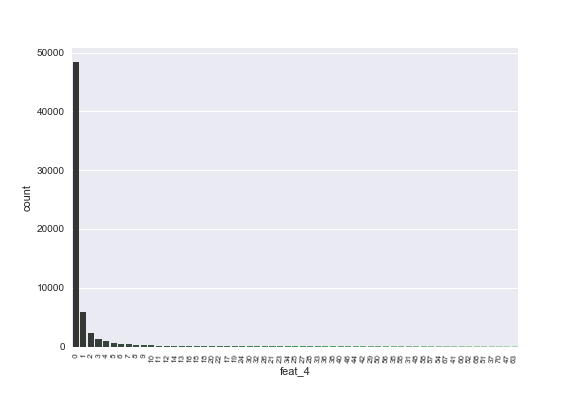
\includegraphics[width=\textwidth]{feat_4}
		\caption{Feature 4}
	\end{subfigure}
	\begin{subfigure}{0.22\textwidth}
		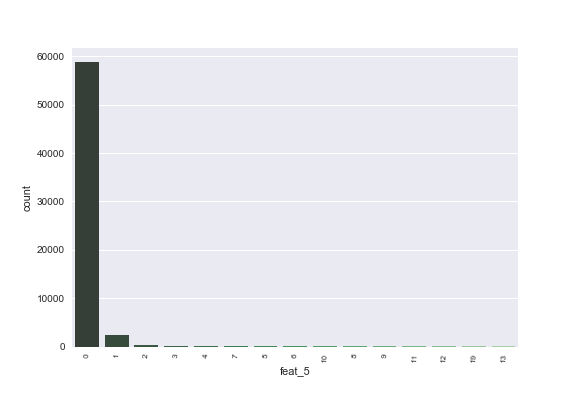
\includegraphics[width=\textwidth]{feat_5}
		\caption{Feature 5}
	\end{subfigure}
	\begin{subfigure}{0.22\textwidth}
		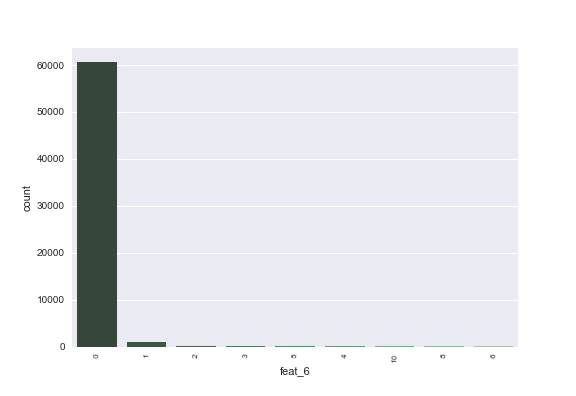
\includegraphics[width=\textwidth]{feat_6}
		\caption{Feature 6}
	\end{subfigure}
	\begin{subfigure}{0.22\textwidth}
		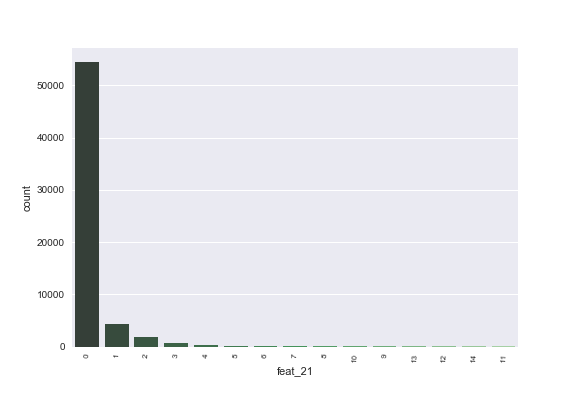
\includegraphics[width=\textwidth]{feat_21}
		\caption{Feature 21}
	\end{subfigure}
		\\
	\begin{subfigure}{0.22\textwidth}
		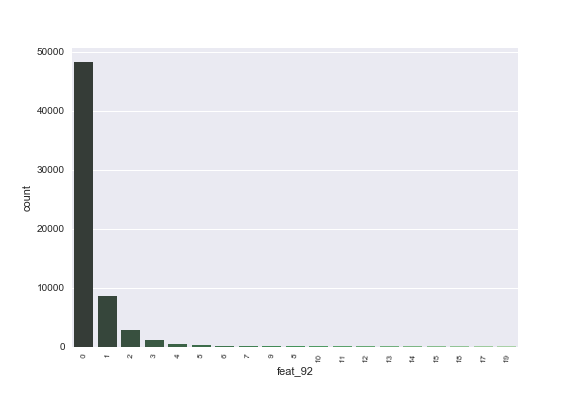
\includegraphics[width=\textwidth]{feat_92}
		\caption{Feature 92}
	\end{subfigure}	
	\begin{subfigure}{0.22\textwidth}
		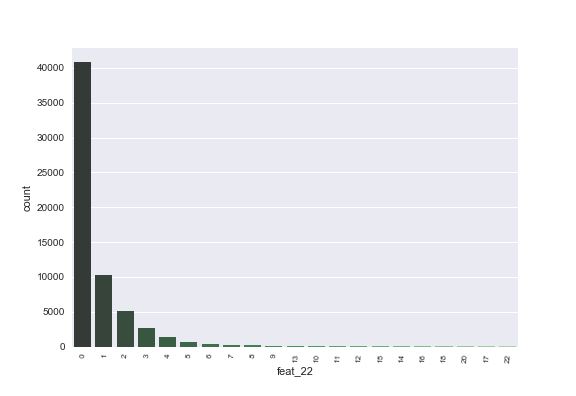
\includegraphics[width=\textwidth]{feat_22}
		\caption{Feature 22}
	\end{subfigure}	
	\begin{subfigure}{0.22\textwidth}
		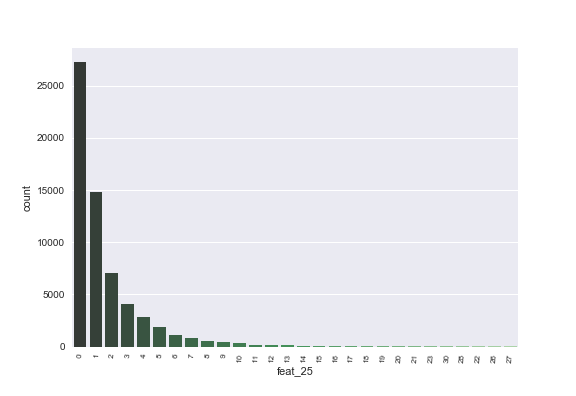
\includegraphics[width=\textwidth]{feat_25}
		\caption{Feature 25}
	\end{subfigure}	
	\begin{subfigure}{0.22\textwidth}
		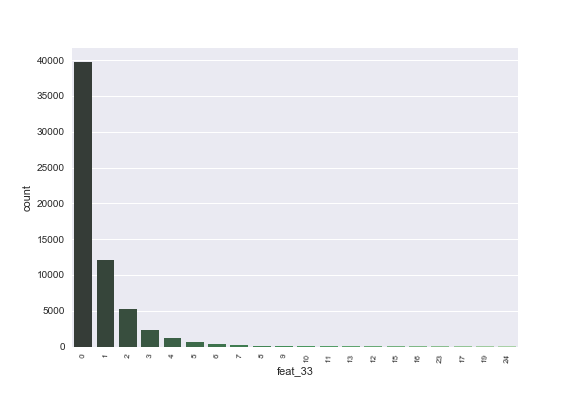
\includegraphics[width=\textwidth]{feat_33}
		\caption{Feature 33}
	\end{subfigure}	
	\caption{Categories distribution for some features}
	\end{figure}


The dominance of the zero class is probably due to unknown features values that has been just transformed to 0.

\subsection{Features correlation}
The correlation study that we did on features reveals that there's no remarkable correlation between them. The more blue is the region, the more correlated the features are. 

\begin{figure}[H]
	\centering
	\includegraphics[width=0.6\textwidth,keepaspectratio]{corr}
	\caption{Correlation between features}
\end{figure}

\subsection{Classes distribution}

As the features categories are not balanced, the problem classes are not balanced too! We see that some classes figure most of time, but this in not the case for the other classes. This makes classification problem more difficult.

\begin{figure}[H]
	\centering
	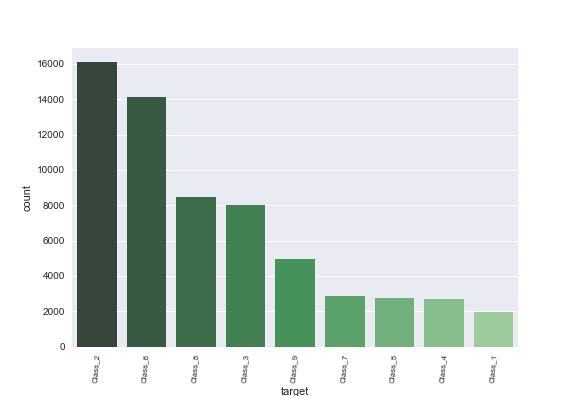
\includegraphics[width=0.8\textwidth,keepaspectratio]{target}
	\caption{Classes distribution in the dataset}
\end{figure}

\section{Classification process}

Because the classes are not balanced, we aimed to devide the dataset in such a way that we keep the same pourcentage of each classe in both train and test sets. The figures below show the result of classes distribution before and after deviding the dataset.

\begin{figure}[H]
	\centering
	\begin{subfigure}{0.22\textwidth}
		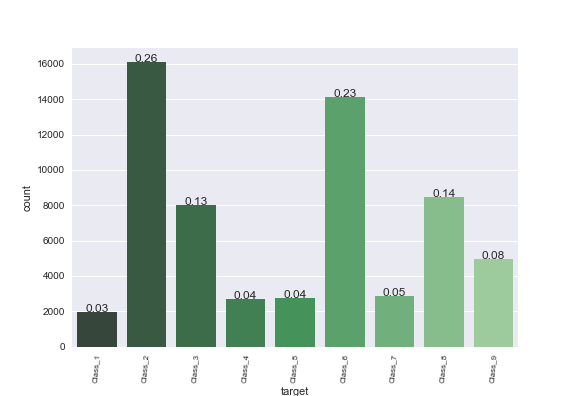
\includegraphics[width=\textwidth]{target_init}
		\caption{Full dataset}
	\end{subfigure}
	\begin{subfigure}{0.22\textwidth}
		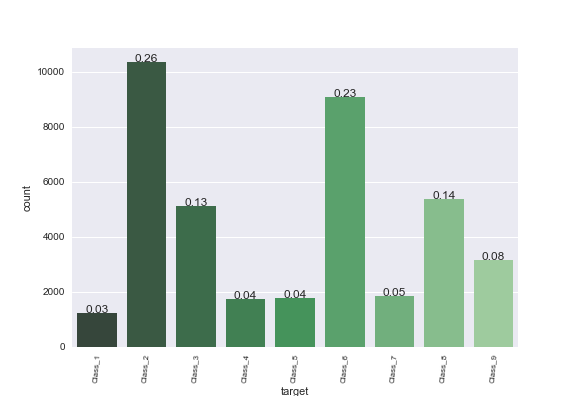
\includegraphics[width=\textwidth]{target_train}
		\caption{Train set}
	\end{subfigure}
	\begin{subfigure}{0.22\textwidth}
		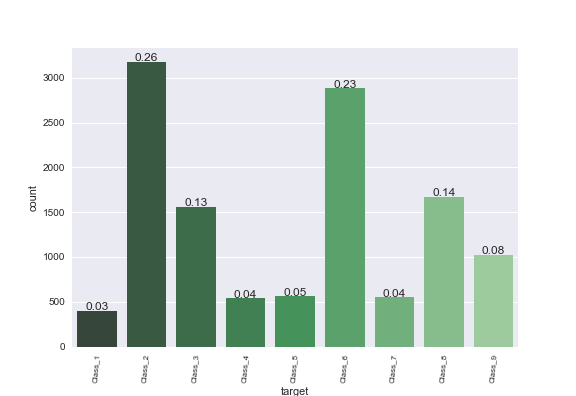
\includegraphics[width=\textwidth]{target_test}
		\caption{Test set}
	\end{subfigure}
	\begin{subfigure}{0.22\textwidth}
		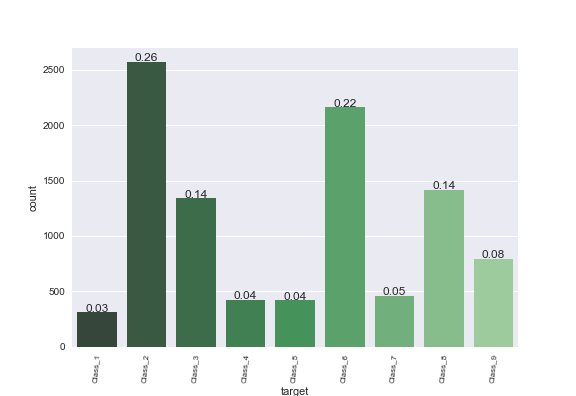
\includegraphics[width=\textwidth]{target_val}
		\caption{Validation set}
	\end{subfigure}
	\caption{Classes distribution for different sets}
\end{figure}

\section{Conclusion}
This is a conclusion

%%%%%%%%%%%%%%%%%%%%%%%%%%%%%%%%%%%%%%%%%%%%%%%%%%%%%%%%%%%%%
\bibliographystyle{babplain}
\parskip=-1em
%\emptypage{\bibliography{bibliographie}}
\let\section\oldsection % pour éviter que le résumé soient visibles dans le sommaire comme une section
%\include{Resume}
\end{document}
